\documentclass[a4paper]{article}

%% Language and font encodings
\usepackage[english]{babel}
\usepackage[utf8x]{inputenc}
\usepackage[T1]{fontenc}

%% Sets page size and margins
\usepackage[a4paper,top=3cm,bottom=2cm,left=3cm,right=3cm,marginparwidth=1.75cm]{geometry}

%% Useful packages
\usepackage{amsmath}
\usepackage{graphicx}
\usepackage[colorinlistoftodos]{todonotes}
\usepackage[colorlinks=true, linkcolor=blue, filecolor=magenta, urlcolor=cyan,]{hyperref}

\title{Kaggle Competition: House Price - Project Report}
\author{Team Golden Squirrels: Lingjie Qiao, Minsu Kim, Kevin Liao, Cheng Peng}

\usepackage{Sweave}
\begin{document}
\Sconcordance{concordance:report.tex:report.Rnw:%
1 19 1 1 0 70 1}

\maketitle

\begin{flushleft}
\begin{abstract}

This paper summarizes the background, problem, methodology and results of our team's final project in the course Stats 159 Reproducible and Collaborative Statistical Data Science. To make full use of statistical models and predictive tools we have learned from the class and challenge ourselves to the next level, our team choose to complete \textbf{"House Price: Advanced Regression Techniques"} from Kaggle Competition and enter the competition with our work. \newline

\textbf{Competition Link:} https://www.kaggle.com/c/house\hspace{0pt}prices\hspace{0pt}advanced\hspace{0pt}regression\hspace{0pt}techniques \newline

The goal of this project is to present the use of predictive modeling process and utilize software tools that effectively communicate the results. While the competition only emphasizes the accuracy of predicted values, our team at the same time are dedicated to maintain project reproducibility and provide both objective and personal reflections upon regression analysis. \newline
\end{abstract}

\section{Introduction}
The House Price project thoroughly explores the predictive modeling process and advanced regression techniques. From previous study, in order to understand the relationship of one dependent variable with several independent variables, we fit a multiple linear regession with Ordinary Least Squares. However, since OLS may have high variance and include irrelevant variables, Predictive Modeling Process can improve the results in terms of \textbf{\textit{Prediction Accuracy}} and \textbf{\textit{Model Interpretability}}. \newline

The competition sets the background of the project: Ask a home buyer to describe their dream house, and they probably won't begin with the height of the basement ceiling or the proximity to an east-west railroad. But this playground competition's dataset proves that much more influences price negotiations than the number of bedrooms or a white-picket fence. \newline

With 79 explanatory variables describing (almost) every aspect of residential homes in Ames, Iowa, this competition requires participants to predict the final price of each home. Our team therefore follows the idea of model prediction and tries to use different techniques in order to most accurately predict the final sales price of each house. \newline


\section{Data}

The datasets are obtained from the Kaggle Competition website. We have access to four files: \newline
1. \textit{data description}, which gives the official definition for fields \newline
2. \textit{train.csv}, which provides 1459 real observations that can be used for model construction \newline
3. \textit{test.csv}, which is used to fit the predictive model and create submission entry for the final sales price of 1460 observations \newline
4. \textit{sample submission}, which gives an example of how the fitted values should be submitted. \newline

The train dataset has in total 80 variables, 79 potential predictors and 1 dependent variable called \textit{SalePrice}. We observe both categorial predictors, such as \textit{FireplaceQu}, \textit{GarageCond} and \textit{MasVnrType} as well as numerical predictors, such as \textit{PoolArea}, \textit{EnclosedPorch} and \textit{YrSold}. Since we can potentially create a lot of different new variables, our goal is to understand the relationship between \textit{SalePrice} and these predictors with statistical fitting procedures that minimizes Mean Square Error.


\section{Methodology}

The goal of this analysis is to accurately predict the final price of each home. Therefore, we frame this problem as a regression problem, and decide to use the L2 loss function [10] which is often used in regression problem. Taking this objective into account, we preprocess original dataset so that regression models can work well. Furthermore, we extract more features by involving feature engineering. Finally, we fit two shrinkage models and two ensemble models. The details are explained in the following subsections.

\subsection{Objective Loss Function}

We specifically use root mean squared logarithmic error [5], which makes more sense in our problem setting because errors in predicting expensive houses and cheap houses should affect the result equally. The following is the formula of RMSLE. \newline

$$
\epsilon = \sqrt{\frac{1}{n} \sum_{i=1}^{n} (log(p_{i} + 1) - log(a_{i} + 1))^2}
$$

Since L2 loss function minimizes the squared differences between the estimated and existing target values [10], L2 error will be much larger in the case of outlier compared to L1 and therefore L2 loss function is highly sensitive to outliers in the dataset. So, in the preprocessing step, we eliminate outliers to remedy this issue. \newline


\section{Analysis}
With the presented methodology, we took the following steps to approach our analysis and presented our results in the subsequent sections.

\subsection{Preprocess}
According to the exploratory data analysis, we find a lot of \textbf{NA values} in most of predictors. Since regression models cannot handle missing data, we need to either remove or impute data using appropriate methods [7]. The data description provided by client [6] indicates that some of the missing values are actually none value. In that case, we replace \textbf{NA} value with factor variable named \textbf{None}. However, there are some numerical predictors with missing values in an unsystematical manner. In that case, we impute them with \textbf{mean values} of predictors. \newline

As a next step, we apply \textbf{log transformations} to \textbf{area related predictors} such as GrLivArea and LotArea as well as target variable. The log transformation has an effect to remedy skewness of data [8] by making original distributions of predictors to more normally distributed. Consequently, it helps regression model to work better. \newline

\begin{figure}[h]
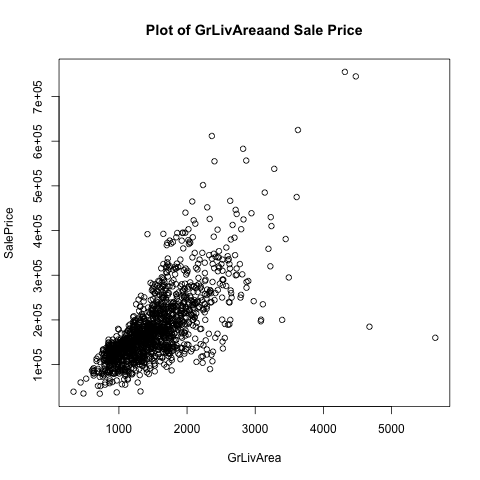
\includegraphics[width=8cm]{../images/plot-GrLivArea.png}
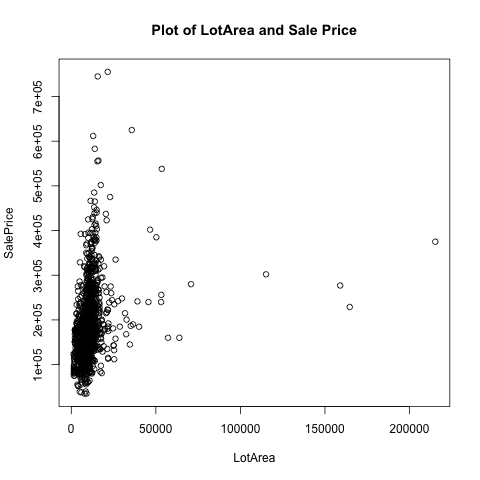
\includegraphics[width=8cm]{../images/plot-LotArea.png}
\end{figure}

After the log transformation, we still notice few outliers and eliminate lowest and highest 0.1\% data points. Furthermore, majority of predictors are categorical under which regression models cannot be used directly. Therefore, we apply \textbf{one-hot encoding} [9] to convert categorical values to numerical ones. It consequently expands features from 79 to approximately 500. The Table 1 below summarizes this procedure. \newline

Table 1: Data Preprocess and Variable Transformation

\vspace{2mm}
\begin{center}
\begin{tabular}{ | p{4.5cm} | p{4.5cm} | p{4.5cm} |}
  \hline			
  Factorization & Log Transformation & Removing Outliers\\
  \hline  
  MSSubClass & SalePrice & 17 points -> below 10.91511 \\
  YearBuilt & LotArea & and above SalePrice \\
  YrSold & GrLivArea & \\ 
  MoSold & & \\
  GarageYrBlt & & \\
  \hline  
\end{tabular}
\end{center}

\subsection{Data Preparation}
Before fitting the model, we first split dataset into train and test. We could have a separate validation set. However,  R library caret has a built-in cross validation as a generic interface. So it automatically takes care of cross validation. We use train data to train and tune our models using 5-kold cross validation, and later compare RMSLE using hold-out test data [13]. \newline

\subsection{Featuring Engineering}

Considering the complexity of the problem as well as the number of observations and predictors, we assume that the success of this analysis is largely dependent on \textbf{informative, feature engineered predictors} that can reveal the subtle relationship to our target variable. Given the small size of dataset with 1460 observations, we conclude that feature learning, which is a set of techniques that learn a \href{https://en.wikipedia.org/wiki/Feature_(machine_learning)}{feature}: a transformation of raw data input to a representation that can be effectively exploited in machine learning tasks [1], is not a feasible option because feature learning often involves very complicated models with multiple layers, which tends to cause an overfitting issue when dataset is small [3]. \newline

With this observation, we therefore focus more on \textbf{manual feature engineering} [4]. This process is a important stepping-stone in that it helps reveal significant predictors that are previously not represented well in original dataset. By explicitly designing what the input x's should be, our predictive models can solve a problem easily. \newline


\subsection{Modeling}
We utilize both \textbf{shrinkage regression models} and \textbf{ensemble models}. Practitioners often favor ensemble models [11] due to their conveniences. Ensemble models such as Random Forest [12], which uses the averaged result from the randomly grown decision trees such as CART [13], often work well with unscaled, missing data and are used for both classification and regression problems. Also, since our dataset contains a hug number of predictors, shrinkage methods such Lasso and Ridge regressions [13], which penalize predictors by shrinking their weights, can be highly effective. Furthermore, we utilize a dimension reduction technique called PCA[13] in order to compress information into lower dimension. The results of modeling will be further explained in the following section in detail.


\section{Results}

We fit shrinkage regression models and ensemble model, experiment the several methods including dimension reduction techniques, feature importance measures. \newline

Figure named (model\_ lasso\_ lambda.png) shows that MSE exponentially increases as log(lambda) values increases. The optimal lambda that minimizes MSE turns out to be 0.02020202. 


\section{Conclusion}

In conclusions, while participating in the Kaggle competition - "House Price: Advanced Regression Techniques", we get a chance to dig down into real-life dataset that have complicated variables, missing values and large number of data entries. Based our analysis on the train dataset, we try to find the regression model and advanced techniques that most accurately predict the housing price, and use the exact model to predict new entries from test file. Exploring and creating visualization of data, we compare the usage of different regression models to understand the relationship between dependent variable \textit{SalePrice} and 79 potential predictors. Fortunately, we ranked No.10 among all 2000 participating teams with our prediction, which not only shows the precision of our own predictive model, but also suggests room of improvement and growth. \newline

This course gives us great opportunity to practice \textbf{project reproducibility}, \textbf{advanced statistical model learning} and \textbf{teamwork delegation}. By deligating work to each team mate and implementing the model to generate results, we aim to maintain project reproducibility and publicity so that more people can learn from our model and benefit for future researches. \textit{If you have any questions or concerns regarding any part of our analysis, please feel free to contact the authors for further clarification.} \newline

\end{flushleft}
\end{document}
